\setlength{\footskip}{8mm}

\chapter{Methodology}
\label{ch:methodology}

\textit{The different components of the proposed system and how they work together are described in this chapter.}

\section{System Overview}
The system will use multiple drones with PixHawk flight controllers, each paired with an individual companion computer and a ground control station (GCS). The operator will set the origin of the global map and select a region of interest on the GCS using Mapviz, a ROS package. The system will then create a grid over the region of interest and calculate paths for the drones. After the expected paths are calculated, the system will calibrate the drones by finding an accurate transformation between each drone's local frame of reference and the global frame. To accomplish this, the drones will move in a predefined flight path while the transformations between each local map of and the global map is refined. After calibration is complete, the system coordinates the flights of the drones as they move along the path the system calculated ensuring coverage of the region of interest. While flying their paths, the drones will stream images from their cameras to the GCS. On the GCS, the SfM module will receive the images and construct an aerial map (a textured 3D mesh) with respect to the global map frame for the region of interest initially selected by the operator.

All the components will be run on a single computer while simulating the system. In simulation mode, PX4 will be run in software in the loop (SITL) mode. Gazebo will be used to visualize the physical world and render simulated video feeds. Network Simulator 3 (NS3) will be used to simulate the networking functions of the wireless mesh network.

\section{System Design}

The different compomenets comprising the system are described here.

\subsection{Components}

The system can be divided into two domains, one comprising the components in the drones, and the other comprising the components in the GCS. Components running on drones will not share information with other drones; they will only share with the GCS. These components will be involved with vehicle platform manipulation and forwarding the video stream. The components on the GCS will be involved with aerial mapping from the video stream received, getting the initial region of interest from the operator, planning the path of each drone, and coordinating the movement of each drone during plan execution.

The flight controller will be installed with PX4 firmware execution. The companion computers and the GCS will run Ubuntu or Raspbian Linux with their Robot Operating System (ROS) installed and will be connected to a wireless mesh network through the IEEE 802.11 devices.

The components on the GCS are:
\begin{itemize}
  \item Robot Operating System: All the components will be designed and implemented with ROS as the base infrastructure. This will give access to the plethora of ROS tools and packages.
  \item Structure from Motion: The aerial map from the video feed of the drones will be constructed by this component.
  \item mapviz: Mapviz is a ROS-based visualization tool with a plug-in system focused on visualization of 2D data. It shows tiled maps using the Microsoft Bing Maps API and has plugins to select polygons on the map, show markers, show NavSat data, among other features that fit the requirements of this system. Mapviz also allows us to fix the origin of the global map.
  \item pegasus\_planner: A new multi-agent path planning ROS node designed for the project.
  \item pegasus\_controller: A new ROS node that will calculate and maintain translations between different map frames, monitor links with the drones, transmit path planning information to the drones, and coordinate the drones during flight.
\end{itemize}

The components in the drones are:
\begin{itemize}
  \item Flight Controller: The drones will use Pixhawk flight controllers with PX4 as their firmware.
  \item Companion Computer: The companion computer will control the flight controller in OFFBOARD mode.
  \item Robot Operating System: The software components will be designed and implemented as ROS nodes.
  \item mavros: The companion computer will use mavros, a ROS package for MavLink communication between companion computers, and flight controllers, to control the flight controller in OFFBOARD.
  \item pegasus\_commander: A new ROS node designed for the project that receives paths and control messages from the GCS. It will also send local poses, GPS positions, flight controller status updates, and GCS link monitoring information.
  \item video streamer: The video feed from the onboard camera will be captured and streamed to the GCS by this component.
\end{itemize}

Figure \ref{fig:system-overview} illustrates the different components of the system controlling three drones.

\begin{figure} \label{fig:system-overview}
  \centering
  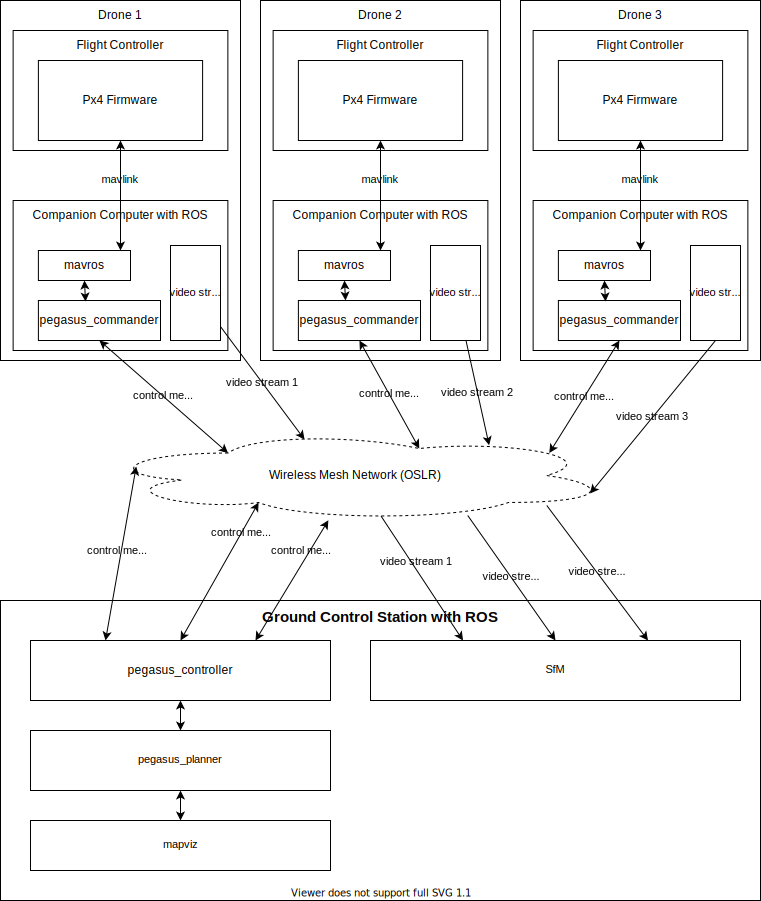
\includegraphics[width=5in]{figures/methodology/system-overview}
  \caption[Pegasus System Overview]{\small Pegasus system overview with three drones.}
\end{figure}


The operator will select the global map origin and region of interest through mapviz. The pegasus\_planner will create a grid-based representation of the region of interest and plan the paths for the drones in the global map reference frame. The initial position of each drone will be provided by pegasus\_controller  to pegasus\_planner. The path planned by pegasus\_planner will be sent to pegasus\_controller. Pegasus\_controller will run a calibration routine on each of the drones to find the transformation between the local origin of the drone and the global map origin. After calibration completes, pegasus\_controller will transform the paths for the drones from global map to the local map for each drone and send it to the drone. Pegasus\_controller will monitor the link with each drone by sending a periodic heart-beat packet. If a drone does not receive a heart-beat packet for some interval, it will change to Return To Home (RTL) mode and abort its current path. To avoid collision, pegasus\_controller will also maintain a path index counter. Paths are made up of a list of poses. Pegasus\_controller will tell each drone to move to the next pose in its path when all the drones have reached their current goal pose.

The SfM module will receive image streams from the drones, and construct an aerial map with respect to the global map frame for the region of interest selected by the operator.

The drones will use mavros, which exposes MavLink protocol parameters and services as ROS topics and services. Pegasus\_commander will receive commands and path information from the GCS and execute its plan while sending local poses, global GPS positions, and flight controller state information back to the GCS. The video streamer will capture images from the onboard camera, apply GPS tags and send them to the GCS.

\subsection{Ground Control Station}

The GCS will be a computer running Ubuntu, with ROS installed. In my particular case, the GCS has an i7 processor, 16 GB of RAM, and a wireless LAN interface.

\subsubsection{Mapviz}
Mapviz requires the operator to select the global map origin as a ROS parameter. ROS parameters can be set through the rosparams command-line tool, programmatically or in the launch file. In our case, we set the local map origin though the launch file using the ROS package swri\_transform\_util.

\begin{verbatim}
<?xml version="1.0"?>
<launch>
  <node pkg="mapviz" type="mapviz" name="mapviz"></node>
  <node pkg="swri_transform_util" type="initialize_origin.py"
    name="initialize_origin" >
    <param name="local_xy_frame" value="/map"/>
    <param name="local_xy_origin" value="control_station"/>
    <rosparam param="local_xy_origins">
      [{
        name: control_station,
        latitude: 14.081104,
        longitude: 100.612743,
        altitude: 7,
        heading: 0.0
      }]
    </rosparam>
  </node>
</launch>
\end{verbatim}

\begin{figure} \label{fig:mapviz-screenshot}
  \centering
  \includegraphics[width=5in]{figures/methodology/gcs/mapviz/screenshot}
  \caption[Mapviz visualizer]{\small Mapviz visualizer with origin set near CSIM.}
\end{figure}

It will publish two ROS topics:
\begin{itemize}
  \item /local\_xy\_origin: Origin of the global map.
  \item /mapviz/region\_selected: The points of the polygon as selected by the user.
\end{itemize}

\subsubsection{Pegasus\_planner}

Pegasus\_planner will handle the following tasks:
\begin{itemize}
  \item Generate grid cells in the region of interest.
  \item Try to calculate the optimal paths for each drone, such that they avoid collisions and stay within the constraints of the wireless mesh network in the global map frame.
\end{itemize}

To generate a valid grid inside the region of interest, consider a polygon with $n$ vertices:

\begin{figure} \label{fig:pegasus-planner-generate-grid-polygon}
  \centering
  \includegraphics[width=4in]{figures/methodology/pegasus_planner/generate_grid/polygon}
  \caption[Polygon Showing the Area of Interest]{\small Polygon showing the area of interest.}
\end{figure}

$$
\text{polygon} = \begin{bmatrix}
  x^0 & y^0 \\
  x^1 & y^1 \\
  x^3 & y^2 \\
  \vdots  & \vdots \\
  x^{n-1} & y^{n-1} \\
\end{bmatrix}. 
$$

The vertices are arranged counter-clockwise/clockwise. To find the bounding box of the polygon, we need to find the vertices.

$$
\text{boundingBox} = \begin{bmatrix}
  x_{min} & y_{min} \\
  x_{max} & y_{min} \\
  x_{max} & y_{max} \\
  x_{min} & y_{max}
\end{bmatrix},
$$

\begin{figure} \label{fig:pegasus-planner-generate-grid-bounding-box}
  \centering
  \includegraphics[width=4in]{figures/methodology/pegasus_planner/generate_grid/bounding-box}
  \caption[Bounding Box on the Polygon Showing the Area of Interest]{\small Bounding box on the Polygon showing the area of interest.}
\end{figure}

where each row defines a vertex. Consider a grid with $n$ cells either horizontally or vertically. Let $c$ be the grid cell size.

$$c = \text{BoundingBox}_{width|heigh} \div  n $$

Alternatively, we can set a fixed size for each cell, or calculate the cell size from camera parameters and the altitude of the drone.

We can then calculate the coordinates $(b^{i,j}_x, b^{i,j}_y)$ of the bottom left vertex of each cell.

$$\text{cells} =\begin{bmatrix}
  b^{0,0}_x & b^{0,0}_y \\
  b^{1,0}_x & b^{1,0}_y \\
  b^{2,0}_x & b^{2,0}_y \\
  \vdots & \vdots \\
  b^{i_{max} - 1,0}_x & b^{i_{max} - 1,0}_y \\
  b^{0,1}_x & b^{0,1}_y \\
  b^{1,1}_x & b^{1,1}_y \\
  b^{2,1}_x & b^{2,1}_y \\
  \vdots & \vdots \\
  b^{i_{max} - 1,0}_x & b^{i_{max} - 1,0}_y \\
  \vdots & \vdots \\
  b^{i_{max} - 1,j_{max}-1}_x & b^{i_{max} - 1,j_{max} - 1}_y \\
\end{bmatrix}$$

$$b^{i,j}_x = x_{min} + i * c$$
$$b^{i,j}_y = y_{min} + j * c$$

$i$, $j$ are the index in $x$  and $y$ axis respectively.


We can get the range of $i$ and $j$ as follows.
$$i_{max} = \left\lceil\frac{x_{max} - x_{min}}{c}\right\rceil $$
$$j_{max} = \left\lceil\frac{y_{max} - y_{min}}{c}\right\rceil$$

Let the number of vertices in $gridCells$ be $k$:
$$ k = i_{max} \times j_{max}.$$


We can then calculate grid index $(i,j)$ from $[0, k]$:

$$j = \left\lfloor\frac{k}{i_{max}}\right\rfloor$$
$$i = k  - j \times i_{max}.$$

\begin{figure} \label{fig:pegasus-planner-generate-cells}
  \centering
  \includegraphics[width=4in]{figures/methodology/pegasus_planner/generate_grid/cells}
  \caption[Cells in the Bounding Box]{\small Bottom left position of the cells in the bounding box.}
\end{figure}

Since the vertex $v$ of the polygon is arranged counter-clockwise/clockwise, we can easily get the vertices of line segment for each side of the polygon.

$$v_i = (x_i, y_i)$$
$$s < n$$

$$\text{polygonLineSegments}=\begin{bmatrix}
  v_0 & v_1 \\
  v_1 & v_2 \\
  \vdots & \vdots \\
  v_s & v_{s+1} \\
  \vdots & \vdots \\
  v_{s_{max}-1} & s_0 \\
\end{bmatrix}$$

$$=\begin{bmatrix}
  x_0 & y_0 & x_1 & y_1 \\
  x_1 & y_1 & x_2 & y_2\\
  \vdots && \vdots \\
  x_s & y_s & x_{s+1} & y_{s+1} \\
  \vdots && \vdots \\
  x_{n-1} & y_{n-1} & x_{0} & y_{0} \\
\end{bmatrix}$$

We can imagine that the center of each grid cell projects a line parallel to the $x$ axis till $x_{max} + 1$.

$$\text{cellCenter} = [\text{cells}] +  \frac{c}{2}$$
$$\text{rays} = \begin{bmatrix}
  \text{cellCenter}_x^{0,0} & \text{cellCenter}_y^{0,1} & x_{max} + 1 & \text{cellCenter}_y^{0,1} \\
  \text{cellCenter}_x^{1,0} & \text{cellCenter}_y^{1,1} & x_{max} + 1 & \text{cellCenter}_y^{1,1} \\
  \text{cellCenter}_x^{2,0} & \text{cellCenter}_y^{2,1} & x_{max} + 1 & \text{cellCenter}_y^{2,1} \\
  \vdots && \vdots \\
  \text{cellCenter}_x^{k-1,0} & \text{cellCenter}_y^{k-1,1} & x_{max} + 1 & \text{cellCenter}_y^{k-1,1} \\
\end{bmatrix}
$$
\begin{figure} \label{fig:pegasus-planner-generate-ray}
  \centering
  \includegraphics[width=4in]{figures/methodology/pegasus_planner/generate_grid/ray}
  \caption[Rays projecting from cell centre to $x_{max} + 1$]{\small Rays projecting from cell centre to $x_{max} + 1$.}
\end{figure}

Now we apply ray tracing to check if $cell^{i,j}$ is inside our polygon or not. We count how many intersections each $rays^{i,j}$ makes with all the lines in $polygonLineSegments$. If the number of intersections are even, then the $cell$ is outside the polygon. If the number of intersections are odd, then the $cell$ is inside the polygon. We now have the valid cells that can the drones can traverse.
\begin{figure} \label{fig:pegasus-planner-generate-valid-cells}
  \centering
  \includegraphics[width=4in]{figures/methodology/pegasus_planner/generate_grid/valid-cells}
  \caption[Grid inside the region of interest]{\small Grid cells inside the region of interest.}
\end{figure}

To plan the path for the drones.....

\subsubsection{Pegasus\_controller}

Pegasus\_controller will be responsible for:
\begin{itemize}
  \item Calculating and maintaining the transformations between the local map frames of each drone and the global map frame.
  \item Coordinating and sending control messages to the drones. Refer to section \ref{section:pegasus-commander} for the list of control messages available.
  \item Monitoring the link with the drones by sending heart beat control message.
  \item Publishing local pose, global GPS coordinates and state of each drone, received from pegasus\_commander as ROS topics.
  \item Publishing the transposed pose and transposed GPS position of all the drones in global map frame.
\end{itemize}

It will have the following states:
\begin{itemize}
  \item IDLE: It will not do anything.
  \item OFFBOARD\_MODE: It will send SET\_OFFBOARD control message to the drones and wait for confirmation.
  \item ARMING: It will send SET\_ARM control message to the drones and wait for confirmation.
  \item TAKE\_OFF: It will send TAKEOFF control message with the altitude to the drones.
  \item CALIBRATE: It will send the calibration path to the drones and coordinate the flight of the drone along the calibration path. It will also capture the corresponding local poses and global GPS positions for calculation the map transformations.
  \item GENERATE\_TRANSFORMS: It will generate the transforms between the local map frame of each drone and the global map frame using the corresponding points collected in CALIBRATE state.
  \item RUN: It will transform the path published by pegasus\_planner on ROS topic /pegasus/[agent]/path to each drone local frame, send it to the drones using SET\_PATH control message, and coordinate the drones using GOTO\_PATH\_INDEX control message.
  \item COMPLETE: It will reach this state when the system's execution is complete. Set the drone to Return mode by sending SET\_RTH control message.
\end{itemize}

Algorithm \ref{find-transforms} will be used to find transforms between local map of each drone and the global map.

\renewcommand{\algorithmicrequire}{\textbf{Input:}}
\renewcommand{\algorithmicensure}{\textbf{Output:}}
\renewcommand{\algorithmicforall}{\textbf{for each}}
\begin{algorithm}
  \caption{Find Local To Global Transformation}
  \label{find-transforms}
  \begin{algorithmic}
    \REQUIRE $L$: set of all corresponding local poses
    \REQUIRE $G$: set of all corresponding global GPS positions
    \REQUIRE $O$: global map origin GPS coordinate
    \ENSURE $T$: transformation between local and global map
    \STATE $\widetilde{O} \gets \textsc{Convert-to-UTM}(O)$
    \STATE $\widetilde{G} \gets \textsc{Convert-to-UTM}(G)$
    \STATE $M \gets \widetilde{O} - \widetilde{G}$
    \STATE $\widehat{M} \gets \textsc{Remove-Z-axis}(\widetilde{M})$
    \STATE $\widehat{L} \gets \textsc{Remove-Z-axis}(L)$
    \STATE $H \gets \textsc{Find-Homography}(\widehat{L}, \widehat{M}, \text{RANSAC})$
    \STATE $T \gets \begin{bmatrix}
      H_{1,1} & H_{2,1} & 0 & H_{3,1} \\
      H_{1,2} & H_{2,2} & 0 & H_{3,2} \\
      0 & 0 & 1 & 0 \\
      0 & 0 & 0 & 1
    \end{bmatrix}$

  \end{algorithmic}
\end{algorithm}

\subsection{Drone}

\subsubsection{PX4}
The drone runs PX4 Firmware on the flight controller. The flight controller's movement and altitude can be controlled in Offboard mode through the MAVlink protocol. This mode supports only a very limited set of MAVLink commands.

MAVLink commands supported in Offboard modes are:
\begin{itemize}
  \item SET\_POSITION\_TARGET\_LOCAL\_NED: Control vehicle position.
  \item SET\_ATTITUDE\_TARGET: Control vehicle altitude and orientation.
\end{itemize}

PX4 supports the coordinate frames (coordinate\_frame field): MAV\_FRAME\_LOCAL\_NED and MAV\_FRAME\_BODY\_NED.

A stream of setpoint commands must be received by the vehicle prior to engaging the mode, and in order to remain in the mode (if the message rate falls below 2Hz the vehicle will stop). In order to hold position while in this mode, the vehicle must receive a stream of setpoints for the current position.

Offboard mode requires an active connection to a remote MAVLink system (e.g. companion computer or GCS). If the connection is lost, after a timeout (COM\_OF\_LOSS\_T) the vehicle will attempt to land or perform some other failsafe action. The action is defined in the parameters COM\_OBL\_ACT and COM\_OBL\_RC\_ACT which can be set through mavros' mavparam.

\subsubsection{Mavros}

Mavros is a ROS node that provides ROS interfaces for communication with various autopilots with MAVLink communication protocol.
The ROS services provided by Mavros,  of interest for this system are:
\begin{itemize}
  \item mavros/set\_mode: Required to set mode of the flight controller to Offboard mode.
  \item mavros/cmd/arming: Required to arm the flight controller.
\end{itemize}

The ROS topics published by Mavros, useful for this system are:
\begin{itemize}
  \item mavros/state: Publishes the state of the flight controller.
  \item mavros/local\_position/pose: Publishes pose, i.e. position and orientation of the flight controller in the local frame. Mavros handles the translation between NED and ENU conventions.
  \item mavros/global\_position/global: Publishes the GPS coordinates, i.e. latitude, longitude and altitude of the flight controller.
\end{itemize}

The ROS topics subscribed by Mavros, that this system will use are:
\begin{itemize}
  \item mavros/setpoint\_position/local: Set the pose, i.e. position and orientation that the flight controller is desired to achieve in local frame.
\end{itemize}

\subsubsection{Pegasus\_commander} \label{section:pegasus-commander}

Pegasus\_commander is a new ROS node, customized for this study that uses the topics and services provided by mavros to control the drone in Offboard mode. It receives control messages from the GCS. It also monitors the link between GCS and the drone, and a heart beat control message is not received for a particular duration, then the flight controller is set to Return mode.

The different types of control messages that will be received by pegasus\_commander from GCS are:
\begin{itemize}
  \item HEART\_BEAT: GCS heart beat in regular intervals.
  \item SET\_OFFBOARD: Put the flight controller in Offboard mode.
  \item SET\_RTH: Put the flight controller in Return mode.
  \item SET\_ARM: Arm the flight controller.
  \item TAKEOFF(float): Set the altitude of the drone.
  \item SET\_PATH(pose): Set the path that the drone needs to follow in local map frame.
  \item GOTO\_PATH\_INDEX(int): Set the local position to the pose in the given index.
\end{itemize}

The different types of control messages that will be sent to the GCS are:
\begin{itemize}
  \item HEART\_BEAT\_ACK: Acknowledgment to the GCS's heart beat.
  \item PATH\_INDEX\_REACHED(int, pose): Return the path index and the local pose when the drone reaches the set-point indicated with GOTO\_PATH\_INDEX message from GPS.
  \item SUCCESS(message): Return success confirmation for message from GCS.
  \item FAILED(message): Return fail confirmation for message from GCS.
\end{itemize}

Pegasus\_commander also transmits the state, local pose and GPS coordinated of the drone to the GCS in regular intervals.

\subsubsection{Video Streamer}

The images from the onboard camera of the drone will be captured. Then each image frame will be geo-tagged with the current GPS coordinates from the flight controller and the geo-tagged image feed will be streamed to the GCS.

\subsection{Simulation}

Most of the components will remain the same regardless of whether runnng in simulation or in the real world. The simulation will run in a single computer. Three more components will be utilized to simulate the system:
\begin{itemize}
  \item Gazebo: Gazebo simulator will be used because it supports fleet of drones and camera feed.
  \item Network Simulator 3: NS3 will be used to simulate the wireless mesh network functions.
  \item pegasus-net-sim: A custom NS3 module that will simulate the mobility of the dro\textsc{}nes and push and pop actual control messages and video feed between the drones and the GCS through the simulator. It will also publish the status of each device in the network.
  \item pegasus\_networl\_status\_util\_node: A custom ROS node that will receive noise and signal strength from pegasus-net-sim and publish the signal-to-noise ratio (SNR) value of each drone as ROS topic.
\end{itemize}

\begin{figure} \label{fig:system-simulation-overview}
  \centering
  \includegraphics[width=5in]{figures/methodology/system-simulation-overview}
  \caption[Pegasus Simulation System Overview]{\small Pegasus Simulation System Overview}
\end{figure}

Figure \ref{fig:system-simulation-overview} describes the simulation system schematically.

Gazebo will be used to simulate the world, the drone mechanics and the video feed. Pegasus-net-sim, a Network Simulator 3 custom module will be used to simulate the wireless mesh network. Pegasus-net-sim will receive the model info from Gazebo and update the position of its nodes. Each node in pegasus-net-sim will have NS3PegasusApp, a custom NS3 application installed, which will send and receive packets in the simulated network. Pegasus-net-sim will function as a proxy application that will receive data in one UDP port, simulate it in NS3 and transmit it through another UDP socket. Using the trace feature in NS3, pegasus-net-sim will publish the noise and signal value for each node of the wireless mesh network.

\FloatBarrier
